\documentclass[twoside]{book}

% Packages required by doxygen
\usepackage{fixltx2e}
\usepackage{calc}
\usepackage{doxygen}
\usepackage[export]{adjustbox} % also loads graphicx
\usepackage{graphicx}
\usepackage[utf8]{inputenc}
\usepackage{makeidx}
\usepackage{multicol}
\usepackage{multirow}
\PassOptionsToPackage{warn}{textcomp}
\usepackage{textcomp}
\usepackage[nointegrals]{wasysym}
\usepackage[table]{xcolor}

% Font selection
\usepackage[T1]{fontenc}
\usepackage[scaled=.90]{helvet}
\usepackage{courier}
\usepackage{amssymb}
\usepackage{sectsty}
\renewcommand{\familydefault}{\sfdefault}
\allsectionsfont{%
  \fontseries{bc}\selectfont%
  \color{darkgray}%
}
\renewcommand{\DoxyLabelFont}{%
  \fontseries{bc}\selectfont%
  \color{darkgray}%
}
\newcommand{\+}{\discretionary{\mbox{\scriptsize$\hookleftarrow$}}{}{}}

% Page & text layout
\usepackage{geometry}
\geometry{%
  a4paper,%
  top=2.5cm,%
  bottom=2.5cm,%
  left=2.5cm,%
  right=2.5cm%
}
\tolerance=750
\hfuzz=15pt
\hbadness=750
\setlength{\emergencystretch}{15pt}
\setlength{\parindent}{0cm}
\setlength{\parskip}{3ex plus 2ex minus 2ex}
\makeatletter
\renewcommand{\paragraph}{%
  \@startsection{paragraph}{4}{0ex}{-1.0ex}{1.0ex}{%
    \normalfont\normalsize\bfseries\SS@parafont%
  }%
}
\renewcommand{\subparagraph}{%
  \@startsection{subparagraph}{5}{0ex}{-1.0ex}{1.0ex}{%
    \normalfont\normalsize\bfseries\SS@subparafont%
  }%
}
\makeatother

% Headers & footers
\usepackage{fancyhdr}
\pagestyle{fancyplain}
\fancyhead[LE]{\fancyplain{}{\bfseries\thepage}}
\fancyhead[CE]{\fancyplain{}{}}
\fancyhead[RE]{\fancyplain{}{\bfseries\leftmark}}
\fancyhead[LO]{\fancyplain{}{\bfseries\rightmark}}
\fancyhead[CO]{\fancyplain{}{}}
\fancyhead[RO]{\fancyplain{}{\bfseries\thepage}}
\fancyfoot[LE]{\fancyplain{}{}}
\fancyfoot[CE]{\fancyplain{}{}}
\fancyfoot[RE]{\fancyplain{}{\bfseries\scriptsize Generated by Doxygen }}
\fancyfoot[LO]{\fancyplain{}{\bfseries\scriptsize Generated by Doxygen }}
\fancyfoot[CO]{\fancyplain{}{}}
\fancyfoot[RO]{\fancyplain{}{}}
\renewcommand{\footrulewidth}{0.4pt}
\renewcommand{\chaptermark}[1]{%
  \markboth{#1}{}%
}
\renewcommand{\sectionmark}[1]{%
  \markright{\thesection\ #1}%
}

% Indices & bibliography
\usepackage{natbib}
\usepackage[titles]{tocloft}
\setcounter{tocdepth}{3}
\setcounter{secnumdepth}{5}
\makeindex

% Hyperlinks (required, but should be loaded last)
\usepackage{ifpdf}
\ifpdf
  \usepackage[pdftex,pagebackref=true]{hyperref}
\else
  \usepackage[ps2pdf,pagebackref=true]{hyperref}
\fi
\hypersetup{%
  colorlinks=true,%
  linkcolor=blue,%
  citecolor=blue,%
  unicode%
}

% Custom commands
\newcommand{\clearemptydoublepage}{%
  \newpage{\pagestyle{empty}\cleardoublepage}%
}

\usepackage{caption}
\captionsetup{labelsep=space,justification=centering,font={bf},singlelinecheck=off,skip=4pt,position=top}

%===== C O N T E N T S =====

\begin{document}

% Titlepage & ToC
\hypersetup{pageanchor=false,
             bookmarksnumbered=true,
             pdfencoding=unicode
            }
\pagenumbering{roman}
\begin{titlepage}
\vspace*{7cm}
\begin{center}%
{\Large Movies }\\
\vspace*{1cm}
{\large Generated by Doxygen 1.8.11}\\
\end{center}
\end{titlepage}
\clearemptydoublepage
\tableofcontents
\clearemptydoublepage
\pagenumbering{arabic}
\hypersetup{pageanchor=true}

%--- Begin generated contents ---
\chapter{Hierarchical Index}
\section{Class Hierarchy}
This inheritance list is sorted roughly, but not completely, alphabetically\+:\begin{DoxyCompactList}
\item \contentsline{section}{com.\+mert.\+Genre}{\pageref{classcom_1_1mert_1_1_genre}}{}
\item \contentsline{section}{com.\+mert.\+test.\+Genre\+Test}{\pageref{classcom_1_1mert_1_1test_1_1_genre_test}}{}
\item \contentsline{section}{com.\+mert.\+test.\+Main\+Servlet\+Test}{\pageref{classcom_1_1mert_1_1test_1_1_main_servlet_test}}{}
\item \contentsline{section}{com.\+mert.\+test.\+Update\+D\+B\+Test}{\pageref{classcom_1_1mert_1_1test_1_1_update_d_b_test}}{}
\item Http\+Servlet\begin{DoxyCompactList}
\item \contentsline{section}{com.\+mert.\+Main\+Servlet}{\pageref{classcom_1_1mert_1_1_main_servlet}}{}
\item \contentsline{section}{com.\+mert.\+Save\+Entries}{\pageref{classcom_1_1mert_1_1_save_entries}}{}
\item \contentsline{section}{com.\+mert.\+Search}{\pageref{classcom_1_1mert_1_1_search}}{}
\item \contentsline{section}{com.\+mert.\+Show\+Entries}{\pageref{classcom_1_1mert_1_1_show_entries}}{}
\item \contentsline{section}{com.\+mert.\+Show\+Movies}{\pageref{classcom_1_1mert_1_1_show_movies}}{}
\item \contentsline{section}{com.\+mert.\+Update\+DB}{\pageref{classcom_1_1mert_1_1_update_d_b}}{}
\end{DoxyCompactList}
\end{DoxyCompactList}

\chapter{Class Index}
\section{Class List}
Here are the classes, structs, unions and interfaces with brief descriptions\+:\begin{DoxyCompactList}
\item\contentsline{section}{\hyperlink{classplanets_1_1_main_servlet}{planets.\+Main\+Servlet} }{\pageref{classplanets_1_1_main_servlet}}{}
\end{DoxyCompactList}

\chapter{Class Documentation}
\hypertarget{classcom_1_1mert_1_1_genre}{}\section{com.\+mert.\+Genre Class Reference}
\label{classcom_1_1mert_1_1_genre}\index{com.\+mert.\+Genre@{com.\+mert.\+Genre}}


\subsection{Detailed Description}
\begin{DoxyAuthor}{Author}
Mert Basic class for Genres with a constructor that initializes variables. 
\end{DoxyAuthor}


The documentation for this class was generated from the following file\+:\begin{DoxyCompactItemize}
\item 
src/com/mert/Genre.\+java\end{DoxyCompactItemize}

\hypertarget{classcom_1_1mert_1_1_main_servlet}{}\section{com.\+mert.\+Main\+Servlet Class Reference}
\label{classcom_1_1mert_1_1_main_servlet}\index{com.\+mert.\+Main\+Servlet@{com.\+mert.\+Main\+Servlet}}
Inheritance diagram for com.\+mert.\+Main\+Servlet\+:\begin{figure}[H]
\begin{center}
\leavevmode
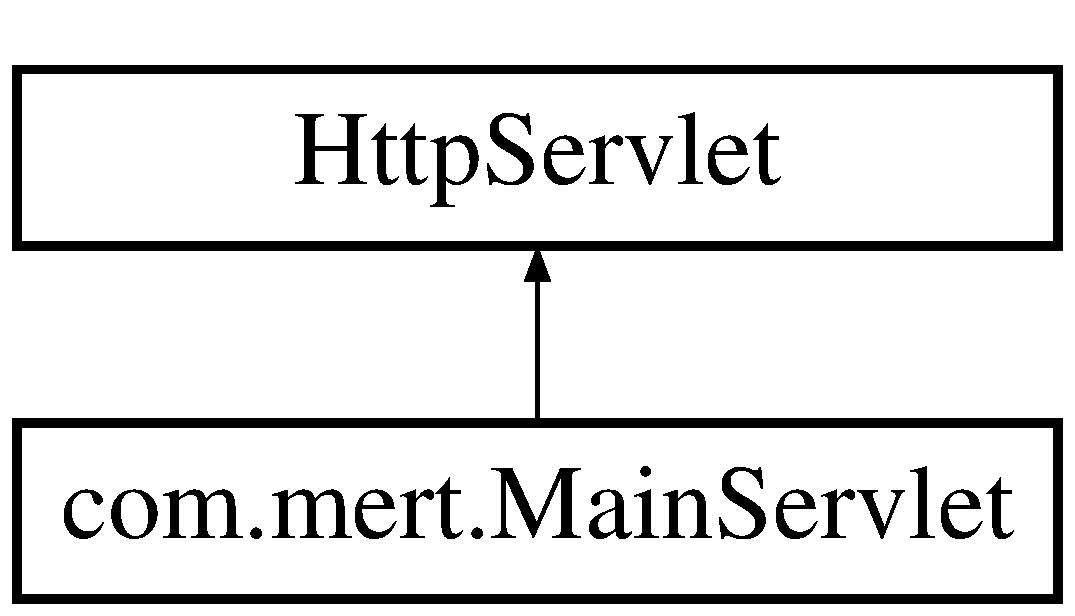
\includegraphics[height=2.000000cm]{classcom_1_1mert_1_1_main_servlet}
\end{center}
\end{figure}
\subsection*{Public Member Functions}
\begin{DoxyCompactItemize}
\item 
\hyperlink{classcom_1_1mert_1_1_main_servlet_a4cd4816907ef657cfb6c7a2403551360}{Main\+Servlet} ()
\item 
void \hyperlink{classcom_1_1mert_1_1_main_servlet_a2f201a8c0bc5b379d4980eae65e774ba}{create\+Movies\+Table} ()
\item 
void \hyperlink{classcom_1_1mert_1_1_main_servlet_a4add4495834801a2cd1aad092e08d2fb}{draw\+Page} (Http\+Servlet\+Request request, Http\+Servlet\+Response response)  throws I\+O\+Exception, Servlet\+Exception, Class\+Not\+Found\+Exception 
\end{DoxyCompactItemize}
\subsection*{Static Public Member Functions}
\begin{DoxyCompactItemize}
\item 
static boolean \hyperlink{classcom_1_1mert_1_1_main_servlet_a44e2c429b5f5c9e74f58d8ec0c044e63}{connect\+To\+DB} ()
\end{DoxyCompactItemize}
\subsection*{Protected Member Functions}
\begin{DoxyCompactItemize}
\item 
void \hyperlink{classcom_1_1mert_1_1_main_servlet_aaff15cf3781104240eb7456c2e249bb5}{do\+Get} (Http\+Servlet\+Request request, Http\+Servlet\+Response response)  throws Servlet\+Exception, I\+O\+Exception 
\item 
void {\bfseries do\+Post} (Http\+Servlet\+Request request, Http\+Servlet\+Response response)  throws Servlet\+Exception, I\+O\+Exception \hypertarget{classcom_1_1mert_1_1_main_servlet_aa028f4c39c100861db897d9d70407249}{}\label{classcom_1_1mert_1_1_main_servlet_aa028f4c39c100861db897d9d70407249}

\end{DoxyCompactItemize}


\subsection{Detailed Description}
\begin{DoxyAuthor}{Author}
Mert Landing page of this web app 
\end{DoxyAuthor}


\subsection{Constructor \& Destructor Documentation}
\index{com\+::mert\+::\+Main\+Servlet@{com\+::mert\+::\+Main\+Servlet}!Main\+Servlet@{Main\+Servlet}}
\index{Main\+Servlet@{Main\+Servlet}!com\+::mert\+::\+Main\+Servlet@{com\+::mert\+::\+Main\+Servlet}}
\subsubsection[{\texorpdfstring{Main\+Servlet()}{MainServlet()}}]{\setlength{\rightskip}{0pt plus 5cm}com.\+mert.\+Main\+Servlet.\+Main\+Servlet (
\begin{DoxyParamCaption}
{}
\end{DoxyParamCaption}
)}\hypertarget{classcom_1_1mert_1_1_main_servlet_a4cd4816907ef657cfb6c7a2403551360}{}\label{classcom_1_1mert_1_1_main_servlet_a4cd4816907ef657cfb6c7a2403551360}
\begin{DoxySeeAlso}{See also}
Http\+Servlet\+::\+Http\+Servlet() 
\end{DoxySeeAlso}


\subsection{Member Function Documentation}
\index{com\+::mert\+::\+Main\+Servlet@{com\+::mert\+::\+Main\+Servlet}!connect\+To\+DB@{connect\+To\+DB}}
\index{connect\+To\+DB@{connect\+To\+DB}!com\+::mert\+::\+Main\+Servlet@{com\+::mert\+::\+Main\+Servlet}}
\subsubsection[{\texorpdfstring{connect\+To\+D\+B()}{connectToDB()}}]{\setlength{\rightskip}{0pt plus 5cm}static boolean com.\+mert.\+Main\+Servlet.\+connect\+To\+DB (
\begin{DoxyParamCaption}
{}
\end{DoxyParamCaption}
)\hspace{0.3cm}{\ttfamily [static]}}\hypertarget{classcom_1_1mert_1_1_main_servlet_a44e2c429b5f5c9e74f58d8ec0c044e63}{}\label{classcom_1_1mert_1_1_main_servlet_a44e2c429b5f5c9e74f58d8ec0c044e63}
Handles all of the sql connections, it is static and is used by other classes too

\begin{DoxyReturn}{Returns}
true if a connection already existed or just established 

false if connection could not be established 
\end{DoxyReturn}
\index{com\+::mert\+::\+Main\+Servlet@{com\+::mert\+::\+Main\+Servlet}!create\+Movies\+Table@{create\+Movies\+Table}}
\index{create\+Movies\+Table@{create\+Movies\+Table}!com\+::mert\+::\+Main\+Servlet@{com\+::mert\+::\+Main\+Servlet}}
\subsubsection[{\texorpdfstring{create\+Movies\+Table()}{createMoviesTable()}}]{\setlength{\rightskip}{0pt plus 5cm}void com.\+mert.\+Main\+Servlet.\+create\+Movies\+Table (
\begin{DoxyParamCaption}
{}
\end{DoxyParamCaption}
)}\hypertarget{classcom_1_1mert_1_1_main_servlet_a2f201a8c0bc5b379d4980eae65e774ba}{}\label{classcom_1_1mert_1_1_main_servlet_a2f201a8c0bc5b379d4980eae65e774ba}
Create movies in local db assuming it does not exist \index{com\+::mert\+::\+Main\+Servlet@{com\+::mert\+::\+Main\+Servlet}!do\+Get@{do\+Get}}
\index{do\+Get@{do\+Get}!com\+::mert\+::\+Main\+Servlet@{com\+::mert\+::\+Main\+Servlet}}
\subsubsection[{\texorpdfstring{do\+Get(\+Http\+Servlet\+Request request, Http\+Servlet\+Response response)}{doGet(HttpServletRequest request, HttpServletResponse response)}}]{\setlength{\rightskip}{0pt plus 5cm}void com.\+mert.\+Main\+Servlet.\+do\+Get (
\begin{DoxyParamCaption}
\item[{Http\+Servlet\+Request}]{request, }
\item[{Http\+Servlet\+Response}]{response}
\end{DoxyParamCaption}
) throws Servlet\+Exception, I\+O\+Exception\hspace{0.3cm}{\ttfamily [protected]}}\hypertarget{classcom_1_1mert_1_1_main_servlet_aaff15cf3781104240eb7456c2e249bb5}{}\label{classcom_1_1mert_1_1_main_servlet_aaff15cf3781104240eb7456c2e249bb5}
This function acts as main and is executed when page is requested.

\begin{DoxySeeAlso}{See also}
Http\+Servlet\+::do\+Get(Http\+Servlet\+Request request, Http\+Servlet\+Response response) 
\end{DoxySeeAlso}
\index{com\+::mert\+::\+Main\+Servlet@{com\+::mert\+::\+Main\+Servlet}!draw\+Page@{draw\+Page}}
\index{draw\+Page@{draw\+Page}!com\+::mert\+::\+Main\+Servlet@{com\+::mert\+::\+Main\+Servlet}}
\subsubsection[{\texorpdfstring{draw\+Page(\+Http\+Servlet\+Request request, Http\+Servlet\+Response response)}{drawPage(HttpServletRequest request, HttpServletResponse response)}}]{\setlength{\rightskip}{0pt plus 5cm}void com.\+mert.\+Main\+Servlet.\+draw\+Page (
\begin{DoxyParamCaption}
\item[{Http\+Servlet\+Request}]{request, }
\item[{Http\+Servlet\+Response}]{response}
\end{DoxyParamCaption}
) throws I\+O\+Exception, Servlet\+Exception, Class\+Not\+Found\+Exception}\hypertarget{classcom_1_1mert_1_1_main_servlet_a4add4495834801a2cd1aad092e08d2fb}{}\label{classcom_1_1mert_1_1_main_servlet_a4add4495834801a2cd1aad092e08d2fb}
Prints out all the html contents on main page such as buttons and search 
\begin{DoxyParams}{Parameters}
{\em request} & \\
\hline
{\em response} & \\
\hline
\end{DoxyParams}

\begin{DoxyExceptions}{Exceptions}
{\em I\+O\+Exception} & \\
\hline
{\em Servlet\+Exception} & \\
\hline
{\em Class\+Not\+Found\+Exception} & \\
\hline
\end{DoxyExceptions}


The documentation for this class was generated from the following file\+:\begin{DoxyCompactItemize}
\item 
src/com/mert/Main\+Servlet.\+java\end{DoxyCompactItemize}

\hypertarget{classcom_1_1mert_1_1_save_entries}{}\section{com.\+mert.\+Save\+Entries Class Reference}
\label{classcom_1_1mert_1_1_save_entries}\index{com.\+mert.\+Save\+Entries@{com.\+mert.\+Save\+Entries}}
Inheritance diagram for com.\+mert.\+Save\+Entries\+:\begin{figure}[H]
\begin{center}
\leavevmode
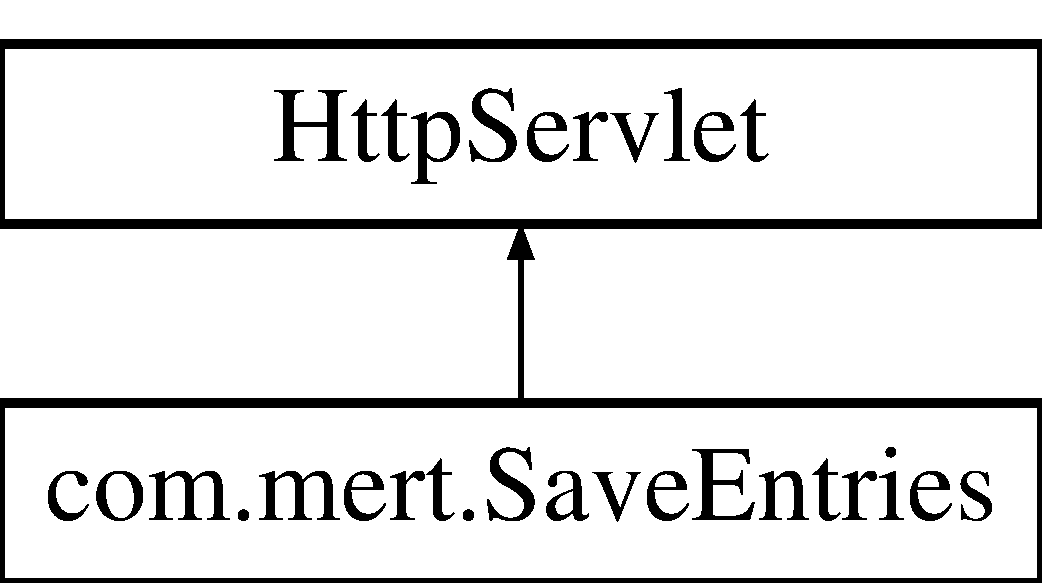
\includegraphics[height=2.000000cm]{classcom_1_1mert_1_1_save_entries}
\end{center}
\end{figure}
\subsection*{Public Member Functions}
\begin{DoxyCompactItemize}
\item 
\hyperlink{classcom_1_1mert_1_1_save_entries_ae19968edd5aa3639abbf947ec2f82caf}{Save\+Entries} ()
\end{DoxyCompactItemize}
\subsection*{Static Public Attributes}
\begin{DoxyCompactItemize}
\item 
static final int {\bfseries M\+Y\+S\+Q\+L\+\_\+\+D\+U\+P\+L\+I\+C\+A\+T\+E\+\_\+\+PK} = 1062\hypertarget{classcom_1_1mert_1_1_save_entries_a00c72d5c09233f18a2ad4f9bf2f28194}{}\label{classcom_1_1mert_1_1_save_entries_a00c72d5c09233f18a2ad4f9bf2f28194}

\end{DoxyCompactItemize}
\subsection*{Protected Member Functions}
\begin{DoxyCompactItemize}
\item 
void \hyperlink{classcom_1_1mert_1_1_save_entries_a5fff9e9797d0c58897db11c3a343f9c4}{do\+Get} (Http\+Servlet\+Request request, Http\+Servlet\+Response response)  throws Servlet\+Exception, I\+O\+Exception 
\item 
void \hyperlink{classcom_1_1mert_1_1_save_entries_ad7a78cb05ce7e6fcbb17e4046d5f2765}{do\+Post} (Http\+Servlet\+Request request, Http\+Servlet\+Response response)  throws Servlet\+Exception, I\+O\+Exception 
\end{DoxyCompactItemize}


\subsection{Detailed Description}
Receives checked I\+Ds by P\+O\+ST method and inserts them into local mysql DB ignores duplicate entries and prints results to html. \begin{DoxyAuthor}{Author}
Mert 
\end{DoxyAuthor}


\subsection{Constructor \& Destructor Documentation}
\index{com\+::mert\+::\+Save\+Entries@{com\+::mert\+::\+Save\+Entries}!Save\+Entries@{Save\+Entries}}
\index{Save\+Entries@{Save\+Entries}!com\+::mert\+::\+Save\+Entries@{com\+::mert\+::\+Save\+Entries}}
\subsubsection[{\texorpdfstring{Save\+Entries()}{SaveEntries()}}]{\setlength{\rightskip}{0pt plus 5cm}com.\+mert.\+Save\+Entries.\+Save\+Entries (
\begin{DoxyParamCaption}
{}
\end{DoxyParamCaption}
)}\hypertarget{classcom_1_1mert_1_1_save_entries_ae19968edd5aa3639abbf947ec2f82caf}{}\label{classcom_1_1mert_1_1_save_entries_ae19968edd5aa3639abbf947ec2f82caf}
\begin{DoxySeeAlso}{See also}
Http\+Servlet\+::\+Http\+Servlet() 
\end{DoxySeeAlso}


\subsection{Member Function Documentation}
\index{com\+::mert\+::\+Save\+Entries@{com\+::mert\+::\+Save\+Entries}!do\+Get@{do\+Get}}
\index{do\+Get@{do\+Get}!com\+::mert\+::\+Save\+Entries@{com\+::mert\+::\+Save\+Entries}}
\subsubsection[{\texorpdfstring{do\+Get(\+Http\+Servlet\+Request request, Http\+Servlet\+Response response)}{doGet(HttpServletRequest request, HttpServletResponse response)}}]{\setlength{\rightskip}{0pt plus 5cm}void com.\+mert.\+Save\+Entries.\+do\+Get (
\begin{DoxyParamCaption}
\item[{Http\+Servlet\+Request}]{request, }
\item[{Http\+Servlet\+Response}]{response}
\end{DoxyParamCaption}
) throws Servlet\+Exception, I\+O\+Exception\hspace{0.3cm}{\ttfamily [protected]}}\hypertarget{classcom_1_1mert_1_1_save_entries_a5fff9e9797d0c58897db11c3a343f9c4}{}\label{classcom_1_1mert_1_1_save_entries_a5fff9e9797d0c58897db11c3a343f9c4}
\begin{DoxySeeAlso}{See also}
Http\+Servlet\+::do\+Get(Http\+Servlet\+Request request, Http\+Servlet\+Response response) 
\end{DoxySeeAlso}
\index{com\+::mert\+::\+Save\+Entries@{com\+::mert\+::\+Save\+Entries}!do\+Post@{do\+Post}}
\index{do\+Post@{do\+Post}!com\+::mert\+::\+Save\+Entries@{com\+::mert\+::\+Save\+Entries}}
\subsubsection[{\texorpdfstring{do\+Post(\+Http\+Servlet\+Request request, Http\+Servlet\+Response response)}{doPost(HttpServletRequest request, HttpServletResponse response)}}]{\setlength{\rightskip}{0pt plus 5cm}void com.\+mert.\+Save\+Entries.\+do\+Post (
\begin{DoxyParamCaption}
\item[{Http\+Servlet\+Request}]{request, }
\item[{Http\+Servlet\+Response}]{response}
\end{DoxyParamCaption}
) throws Servlet\+Exception, I\+O\+Exception\hspace{0.3cm}{\ttfamily [protected]}}\hypertarget{classcom_1_1mert_1_1_save_entries_ad7a78cb05ce7e6fcbb17e4046d5f2765}{}\label{classcom_1_1mert_1_1_save_entries_ad7a78cb05ce7e6fcbb17e4046d5f2765}
\begin{DoxySeeAlso}{See also}
Http\+Servlet\+::do\+Post(Http\+Servlet\+Request request, Http\+Servlet\+Response response) 
\end{DoxySeeAlso}


The documentation for this class was generated from the following file\+:\begin{DoxyCompactItemize}
\item 
src/com/mert/Save\+Entries.\+java\end{DoxyCompactItemize}

\hypertarget{classcom_1_1mert_1_1_search}{}\section{com.\+mert.\+Search Class Reference}
\label{classcom_1_1mert_1_1_search}\index{com.\+mert.\+Search@{com.\+mert.\+Search}}
Inheritance diagram for com.\+mert.\+Search\+:\begin{figure}[H]
\begin{center}
\leavevmode
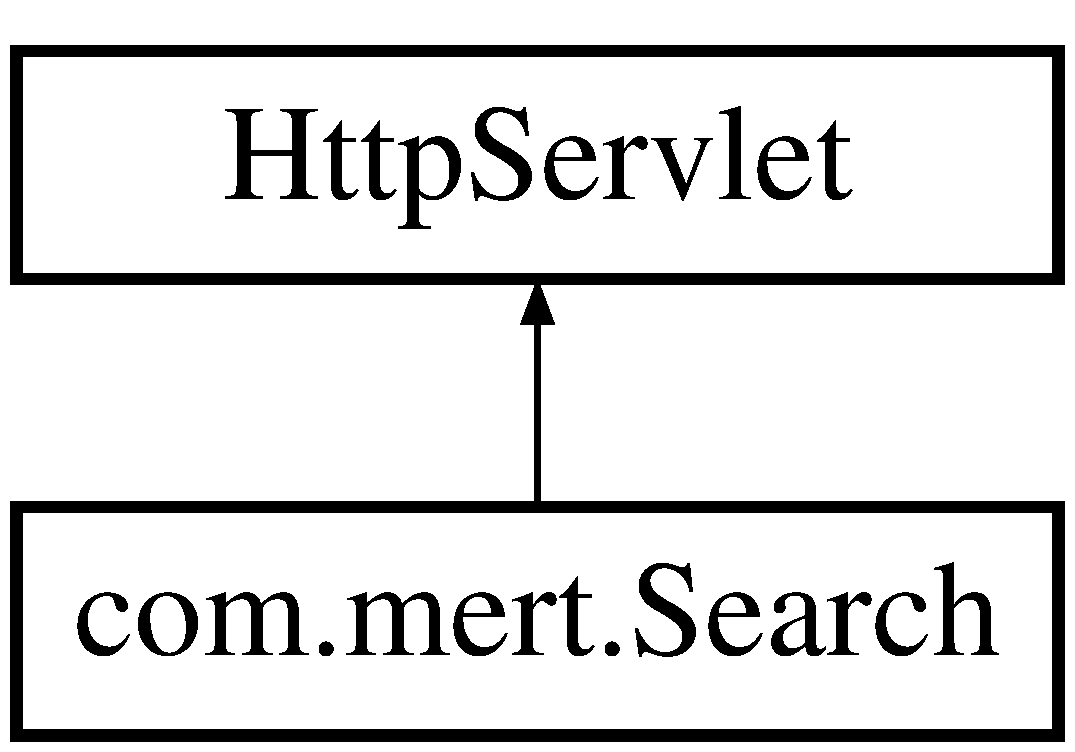
\includegraphics[height=2.000000cm]{classcom_1_1mert_1_1_search}
\end{center}
\end{figure}
\subsection*{Classes}
\begin{DoxyCompactItemize}
\item 
class {\bfseries Comp}
\end{DoxyCompactItemize}
\subsection*{Public Member Functions}
\begin{DoxyCompactItemize}
\item 
\hyperlink{classcom_1_1mert_1_1_search_adb57f5c1f90037b37445e6caddbae989}{Search} ()
\item 
Tree\+Map$<$ String, Integer $>$ {\bfseries sort\+Results} (Array\+List$<$ String $>$ found\+At)\hypertarget{classcom_1_1mert_1_1_search_a0ad68f9506cfbba9d149930d76aceca6}{}\label{classcom_1_1mert_1_1_search_a0ad68f9506cfbba9d149930d76aceca6}

\item 
Array\+List$<$ String $>$ \hyperlink{classcom_1_1mert_1_1_search_a07fd75951344d799a0b03eff2a3d7711}{search\+Array\+List} (Array\+List$<$ Array\+List$<$ String $>$$>$ db, String search\+Term)
\item 
void \hyperlink{classcom_1_1mert_1_1_search_a2c25c0cf503bcc464fea33af4869ac42}{display\+Results} (Tree\+Map$<$ String, Integer $>$ found\+At, Print\+Writer out)
\end{DoxyCompactItemize}
\subsection*{Protected Member Functions}
\begin{DoxyCompactItemize}
\item 
void \hyperlink{classcom_1_1mert_1_1_search_a28593c1902aa8b54f267384d666744d1}{do\+Get} (Http\+Servlet\+Request request, Http\+Servlet\+Response response)  throws Servlet\+Exception, I\+O\+Exception 
\item 
void \hyperlink{classcom_1_1mert_1_1_search_a83f297bcd977985a9f999ae6212168bd}{do\+Post} (Http\+Servlet\+Request request, Http\+Servlet\+Response response)  throws Servlet\+Exception, I\+O\+Exception 
\end{DoxyCompactItemize}


\subsection{Detailed Description}
Creates an arraylist of arraylists that hold Strings( i.\+e 2D String holder data structures) a movie subject from db is split into its words and are inserted into the arraylist.

\begin{DoxyAuthor}{Author}
Mert 
\end{DoxyAuthor}


\subsection{Constructor \& Destructor Documentation}
\index{com\+::mert\+::\+Search@{com\+::mert\+::\+Search}!Search@{Search}}
\index{Search@{Search}!com\+::mert\+::\+Search@{com\+::mert\+::\+Search}}
\subsubsection[{\texorpdfstring{Search()}{Search()}}]{\setlength{\rightskip}{0pt plus 5cm}com.\+mert.\+Search.\+Search (
\begin{DoxyParamCaption}
{}
\end{DoxyParamCaption}
)}\hypertarget{classcom_1_1mert_1_1_search_adb57f5c1f90037b37445e6caddbae989}{}\label{classcom_1_1mert_1_1_search_adb57f5c1f90037b37445e6caddbae989}
\begin{DoxySeeAlso}{See also}
Http\+Servlet\+::\+Http\+Servlet() 
\end{DoxySeeAlso}


\subsection{Member Function Documentation}
\index{com\+::mert\+::\+Search@{com\+::mert\+::\+Search}!display\+Results@{display\+Results}}
\index{display\+Results@{display\+Results}!com\+::mert\+::\+Search@{com\+::mert\+::\+Search}}
\subsubsection[{\texorpdfstring{display\+Results(\+Tree\+Map$<$ String, Integer $>$ found\+At, Print\+Writer out)}{displayResults(TreeMap< String, Integer > foundAt, PrintWriter out)}}]{\setlength{\rightskip}{0pt plus 5cm}void com.\+mert.\+Search.\+display\+Results (
\begin{DoxyParamCaption}
\item[{Tree\+Map$<$ String, Integer $>$}]{found\+At, }
\item[{Print\+Writer}]{out}
\end{DoxyParamCaption}
)}\hypertarget{classcom_1_1mert_1_1_search_a2c25c0cf503bcc464fea33af4869ac42}{}\label{classcom_1_1mert_1_1_search_a2c25c0cf503bcc464fea33af4869ac42}
Receives results of search from the search\+Array\+List function as an Array\+List. Queries wikidata.\+org for movies with the related Main Subjects that were found in search. Lastly prints results of wikidata query to html.


\begin{DoxyParams}{Parameters}
{\em found\+At} & List of search results \\
\hline
{\em out} & Print\+Writer object used to print to html. \\
\hline
\end{DoxyParams}
\index{com\+::mert\+::\+Search@{com\+::mert\+::\+Search}!do\+Get@{do\+Get}}
\index{do\+Get@{do\+Get}!com\+::mert\+::\+Search@{com\+::mert\+::\+Search}}
\subsubsection[{\texorpdfstring{do\+Get(\+Http\+Servlet\+Request request, Http\+Servlet\+Response response)}{doGet(HttpServletRequest request, HttpServletResponse response)}}]{\setlength{\rightskip}{0pt plus 5cm}void com.\+mert.\+Search.\+do\+Get (
\begin{DoxyParamCaption}
\item[{Http\+Servlet\+Request}]{request, }
\item[{Http\+Servlet\+Response}]{response}
\end{DoxyParamCaption}
) throws Servlet\+Exception, I\+O\+Exception\hspace{0.3cm}{\ttfamily [protected]}}\hypertarget{classcom_1_1mert_1_1_search_a28593c1902aa8b54f267384d666744d1}{}\label{classcom_1_1mert_1_1_search_a28593c1902aa8b54f267384d666744d1}
\begin{DoxySeeAlso}{See also}
Http\+Servlet\+::do\+Get(Http\+Servlet\+Request request, Http\+Servlet\+Response response) 
\end{DoxySeeAlso}
\index{com\+::mert\+::\+Search@{com\+::mert\+::\+Search}!do\+Post@{do\+Post}}
\index{do\+Post@{do\+Post}!com\+::mert\+::\+Search@{com\+::mert\+::\+Search}}
\subsubsection[{\texorpdfstring{do\+Post(\+Http\+Servlet\+Request request, Http\+Servlet\+Response response)}{doPost(HttpServletRequest request, HttpServletResponse response)}}]{\setlength{\rightskip}{0pt plus 5cm}void com.\+mert.\+Search.\+do\+Post (
\begin{DoxyParamCaption}
\item[{Http\+Servlet\+Request}]{request, }
\item[{Http\+Servlet\+Response}]{response}
\end{DoxyParamCaption}
) throws Servlet\+Exception, I\+O\+Exception\hspace{0.3cm}{\ttfamily [protected]}}\hypertarget{classcom_1_1mert_1_1_search_a83f297bcd977985a9f999ae6212168bd}{}\label{classcom_1_1mert_1_1_search_a83f297bcd977985a9f999ae6212168bd}
\begin{DoxySeeAlso}{See also}
Http\+Servlet\+::do\+Post(Http\+Servlet\+Request request, Http\+Servlet\+Response response) 
\end{DoxySeeAlso}
\index{com\+::mert\+::\+Search@{com\+::mert\+::\+Search}!search\+Array\+List@{search\+Array\+List}}
\index{search\+Array\+List@{search\+Array\+List}!com\+::mert\+::\+Search@{com\+::mert\+::\+Search}}
\subsubsection[{\texorpdfstring{search\+Array\+List(\+Array\+List$<$ Array\+List$<$ String $>$$>$ db, String search\+Term)}{searchArrayList(ArrayList< ArrayList< String >> db, String searchTerm)}}]{\setlength{\rightskip}{0pt plus 5cm}Array\+List$<$String$>$ com.\+mert.\+Search.\+search\+Array\+List (
\begin{DoxyParamCaption}
\item[{Array\+List$<$ Array\+List$<$ String $>$$>$}]{db, }
\item[{String}]{search\+Term}
\end{DoxyParamCaption}
)}\hypertarget{classcom_1_1mert_1_1_search_a07fd75951344d799a0b03eff2a3d7711}{}\label{classcom_1_1mert_1_1_search_a07fd75951344d799a0b03eff2a3d7711}
The function then compares each word for a match with the searched term. If a match is found its main subject ID is saved to results. It is case sensitive and can not handle small typos.


\begin{DoxyParams}{Parameters}
{\em db} & Named as it holds the info from the database to be searched. \\
\hline
{\em search\+Term} & Entered \\
\hline
\end{DoxyParams}
\begin{DoxyReturn}{Returns}
list of I\+Ds of subjects 
\end{DoxyReturn}


The documentation for this class was generated from the following file\+:\begin{DoxyCompactItemize}
\item 
src/com/mert/Search.\+java\end{DoxyCompactItemize}

\hypertarget{classcom_1_1mert_1_1_show_entries}{}\section{com.\+mert.\+Show\+Entries Class Reference}
\label{classcom_1_1mert_1_1_show_entries}\index{com.\+mert.\+Show\+Entries@{com.\+mert.\+Show\+Entries}}
Inheritance diagram for com.\+mert.\+Show\+Entries\+:\begin{figure}[H]
\begin{center}
\leavevmode
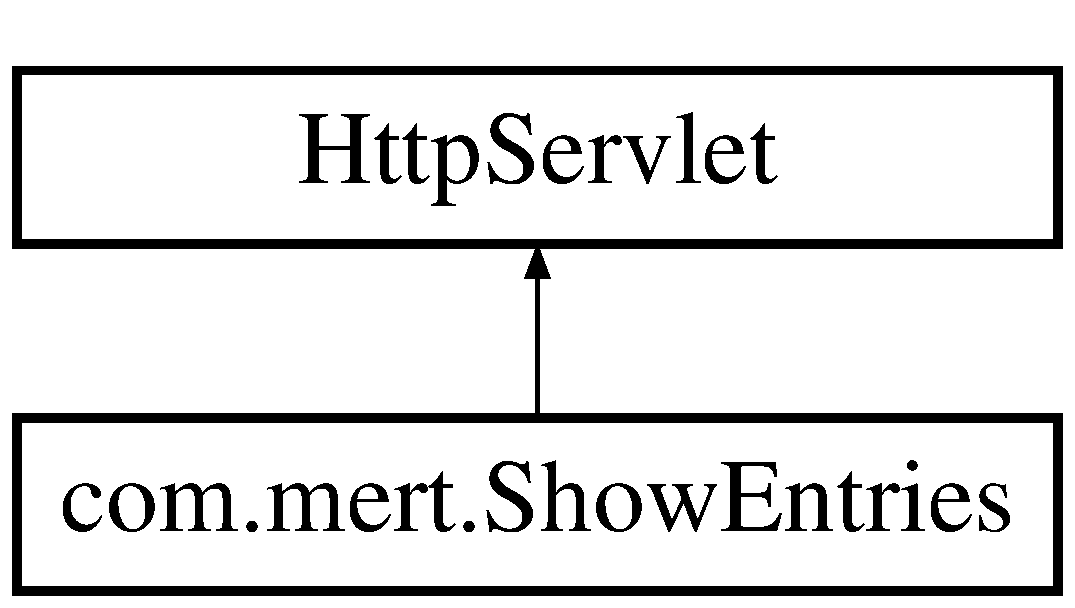
\includegraphics[height=2.000000cm]{classcom_1_1mert_1_1_show_entries}
\end{center}
\end{figure}
\subsection*{Public Member Functions}
\begin{DoxyCompactItemize}
\item 
\hyperlink{classcom_1_1mert_1_1_show_entries_a8eb14533e722559f68c524926574c089}{Show\+Entries} ()
\end{DoxyCompactItemize}
\subsection*{Protected Member Functions}
\begin{DoxyCompactItemize}
\item 
void \hyperlink{classcom_1_1mert_1_1_show_entries_aac85a39ebe42db0bb8b85d1384e4f24f}{do\+Get} (Http\+Servlet\+Request request, Http\+Servlet\+Response response)  throws Servlet\+Exception, I\+O\+Exception 
\item 
void \hyperlink{classcom_1_1mert_1_1_show_entries_a84c2823b4ee4487c4f969932213d5587}{do\+Post} (Http\+Servlet\+Request request, Http\+Servlet\+Response response)  throws Servlet\+Exception, I\+O\+Exception 
\end{DoxyCompactItemize}


\subsection{Detailed Description}
Queries and displays entries stored in local DB Only the ID is stored and is shown. \begin{DoxyAuthor}{Author}
Mert 
\end{DoxyAuthor}


\subsection{Constructor \& Destructor Documentation}
\index{com\+::mert\+::\+Show\+Entries@{com\+::mert\+::\+Show\+Entries}!Show\+Entries@{Show\+Entries}}
\index{Show\+Entries@{Show\+Entries}!com\+::mert\+::\+Show\+Entries@{com\+::mert\+::\+Show\+Entries}}
\subsubsection[{\texorpdfstring{Show\+Entries()}{ShowEntries()}}]{\setlength{\rightskip}{0pt plus 5cm}com.\+mert.\+Show\+Entries.\+Show\+Entries (
\begin{DoxyParamCaption}
{}
\end{DoxyParamCaption}
)}\hypertarget{classcom_1_1mert_1_1_show_entries_a8eb14533e722559f68c524926574c089}{}\label{classcom_1_1mert_1_1_show_entries_a8eb14533e722559f68c524926574c089}
\begin{DoxySeeAlso}{See also}
Http\+Servlet\+::\+Http\+Servlet() 
\end{DoxySeeAlso}


\subsection{Member Function Documentation}
\index{com\+::mert\+::\+Show\+Entries@{com\+::mert\+::\+Show\+Entries}!do\+Get@{do\+Get}}
\index{do\+Get@{do\+Get}!com\+::mert\+::\+Show\+Entries@{com\+::mert\+::\+Show\+Entries}}
\subsubsection[{\texorpdfstring{do\+Get(\+Http\+Servlet\+Request request, Http\+Servlet\+Response response)}{doGet(HttpServletRequest request, HttpServletResponse response)}}]{\setlength{\rightskip}{0pt plus 5cm}void com.\+mert.\+Show\+Entries.\+do\+Get (
\begin{DoxyParamCaption}
\item[{Http\+Servlet\+Request}]{request, }
\item[{Http\+Servlet\+Response}]{response}
\end{DoxyParamCaption}
) throws Servlet\+Exception, I\+O\+Exception\hspace{0.3cm}{\ttfamily [protected]}}\hypertarget{classcom_1_1mert_1_1_show_entries_aac85a39ebe42db0bb8b85d1384e4f24f}{}\label{classcom_1_1mert_1_1_show_entries_aac85a39ebe42db0bb8b85d1384e4f24f}
\begin{DoxySeeAlso}{See also}
Http\+Servlet\+::do\+Get(Http\+Servlet\+Request request, Http\+Servlet\+Response response) 
\end{DoxySeeAlso}
\index{com\+::mert\+::\+Show\+Entries@{com\+::mert\+::\+Show\+Entries}!do\+Post@{do\+Post}}
\index{do\+Post@{do\+Post}!com\+::mert\+::\+Show\+Entries@{com\+::mert\+::\+Show\+Entries}}
\subsubsection[{\texorpdfstring{do\+Post(\+Http\+Servlet\+Request request, Http\+Servlet\+Response response)}{doPost(HttpServletRequest request, HttpServletResponse response)}}]{\setlength{\rightskip}{0pt plus 5cm}void com.\+mert.\+Show\+Entries.\+do\+Post (
\begin{DoxyParamCaption}
\item[{Http\+Servlet\+Request}]{request, }
\item[{Http\+Servlet\+Response}]{response}
\end{DoxyParamCaption}
) throws Servlet\+Exception, I\+O\+Exception\hspace{0.3cm}{\ttfamily [protected]}}\hypertarget{classcom_1_1mert_1_1_show_entries_a84c2823b4ee4487c4f969932213d5587}{}\label{classcom_1_1mert_1_1_show_entries_a84c2823b4ee4487c4f969932213d5587}
\begin{DoxySeeAlso}{See also}
Http\+Servlet\+::do\+Post(Http\+Servlet\+Request request, Http\+Servlet\+Response response) 
\end{DoxySeeAlso}


The documentation for this class was generated from the following file\+:\begin{DoxyCompactItemize}
\item 
src/com/mert/Show\+Entries.\+java\end{DoxyCompactItemize}

\hypertarget{classcom_1_1mert_1_1_show_movies}{}\section{com.\+mert.\+Show\+Movies Class Reference}
\label{classcom_1_1mert_1_1_show_movies}\index{com.\+mert.\+Show\+Movies@{com.\+mert.\+Show\+Movies}}
Inheritance diagram for com.\+mert.\+Show\+Movies\+:\begin{figure}[H]
\begin{center}
\leavevmode
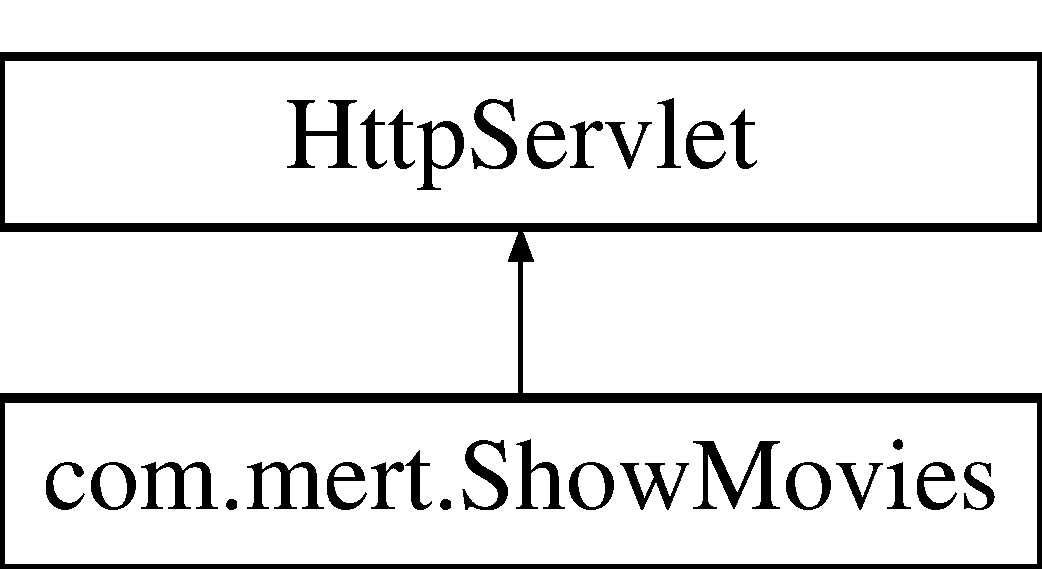
\includegraphics[height=2.000000cm]{classcom_1_1mert_1_1_show_movies}
\end{center}
\end{figure}
\subsection*{Public Member Functions}
\begin{DoxyCompactItemize}
\item 
\hyperlink{classcom_1_1mert_1_1_show_movies_ab55ca7d2cfa298c4bb04072756b652d0}{Show\+Movies} ()
\end{DoxyCompactItemize}
\subsection*{Protected Member Functions}
\begin{DoxyCompactItemize}
\item 
void \hyperlink{classcom_1_1mert_1_1_show_movies_a9fa813716d40b2d43434755e72b20e1f}{do\+Get} (Http\+Servlet\+Request request, Http\+Servlet\+Response response)  throws Servlet\+Exception, I\+O\+Exception 
\item 
void \hyperlink{classcom_1_1mert_1_1_show_movies_a4000ab0c0da1f5e6b501829dd8b2a576}{do\+Post} (Http\+Servlet\+Request request, Http\+Servlet\+Response response)  throws Servlet\+Exception, I\+O\+Exception 
\end{DoxyCompactItemize}


\subsection{Detailed Description}
Receives main subjects I\+DS from local DB and searches wikidata for movies that won oscar with that subject. Prints resulting movies and their subjects as a table \begin{DoxyAuthor}{Author}
Mert 
\end{DoxyAuthor}


\subsection{Constructor \& Destructor Documentation}
\index{com\+::mert\+::\+Show\+Movies@{com\+::mert\+::\+Show\+Movies}!Show\+Movies@{Show\+Movies}}
\index{Show\+Movies@{Show\+Movies}!com\+::mert\+::\+Show\+Movies@{com\+::mert\+::\+Show\+Movies}}
\subsubsection[{\texorpdfstring{Show\+Movies()}{ShowMovies()}}]{\setlength{\rightskip}{0pt plus 5cm}com.\+mert.\+Show\+Movies.\+Show\+Movies (
\begin{DoxyParamCaption}
{}
\end{DoxyParamCaption}
)}\hypertarget{classcom_1_1mert_1_1_show_movies_ab55ca7d2cfa298c4bb04072756b652d0}{}\label{classcom_1_1mert_1_1_show_movies_ab55ca7d2cfa298c4bb04072756b652d0}
\begin{DoxySeeAlso}{See also}
Http\+Servlet\+::\+Http\+Servlet() 
\end{DoxySeeAlso}


\subsection{Member Function Documentation}
\index{com\+::mert\+::\+Show\+Movies@{com\+::mert\+::\+Show\+Movies}!do\+Get@{do\+Get}}
\index{do\+Get@{do\+Get}!com\+::mert\+::\+Show\+Movies@{com\+::mert\+::\+Show\+Movies}}
\subsubsection[{\texorpdfstring{do\+Get(\+Http\+Servlet\+Request request, Http\+Servlet\+Response response)}{doGet(HttpServletRequest request, HttpServletResponse response)}}]{\setlength{\rightskip}{0pt plus 5cm}void com.\+mert.\+Show\+Movies.\+do\+Get (
\begin{DoxyParamCaption}
\item[{Http\+Servlet\+Request}]{request, }
\item[{Http\+Servlet\+Response}]{response}
\end{DoxyParamCaption}
) throws Servlet\+Exception, I\+O\+Exception\hspace{0.3cm}{\ttfamily [protected]}}\hypertarget{classcom_1_1mert_1_1_show_movies_a9fa813716d40b2d43434755e72b20e1f}{}\label{classcom_1_1mert_1_1_show_movies_a9fa813716d40b2d43434755e72b20e1f}
\begin{DoxySeeAlso}{See also}
Http\+Servlet\+::do\+Get(Http\+Servlet\+Request request, Http\+Servlet\+Response response) 
\end{DoxySeeAlso}
\index{com\+::mert\+::\+Show\+Movies@{com\+::mert\+::\+Show\+Movies}!do\+Post@{do\+Post}}
\index{do\+Post@{do\+Post}!com\+::mert\+::\+Show\+Movies@{com\+::mert\+::\+Show\+Movies}}
\subsubsection[{\texorpdfstring{do\+Post(\+Http\+Servlet\+Request request, Http\+Servlet\+Response response)}{doPost(HttpServletRequest request, HttpServletResponse response)}}]{\setlength{\rightskip}{0pt plus 5cm}void com.\+mert.\+Show\+Movies.\+do\+Post (
\begin{DoxyParamCaption}
\item[{Http\+Servlet\+Request}]{request, }
\item[{Http\+Servlet\+Response}]{response}
\end{DoxyParamCaption}
) throws Servlet\+Exception, I\+O\+Exception\hspace{0.3cm}{\ttfamily [protected]}}\hypertarget{classcom_1_1mert_1_1_show_movies_a4000ab0c0da1f5e6b501829dd8b2a576}{}\label{classcom_1_1mert_1_1_show_movies_a4000ab0c0da1f5e6b501829dd8b2a576}
\begin{DoxySeeAlso}{See also}
Http\+Servlet\+::do\+Post(Http\+Servlet\+Request request, Http\+Servlet\+Response response) 
\end{DoxySeeAlso}


The documentation for this class was generated from the following file\+:\begin{DoxyCompactItemize}
\item 
src/com/mert/Show\+Movies.\+java\end{DoxyCompactItemize}

\hypertarget{classcom_1_1mert_1_1_update_d_b}{}\section{com.\+mert.\+Update\+DB Class Reference}
\label{classcom_1_1mert_1_1_update_d_b}\index{com.\+mert.\+Update\+DB@{com.\+mert.\+Update\+DB}}
Inheritance diagram for com.\+mert.\+Update\+DB\+:\begin{figure}[H]
\begin{center}
\leavevmode
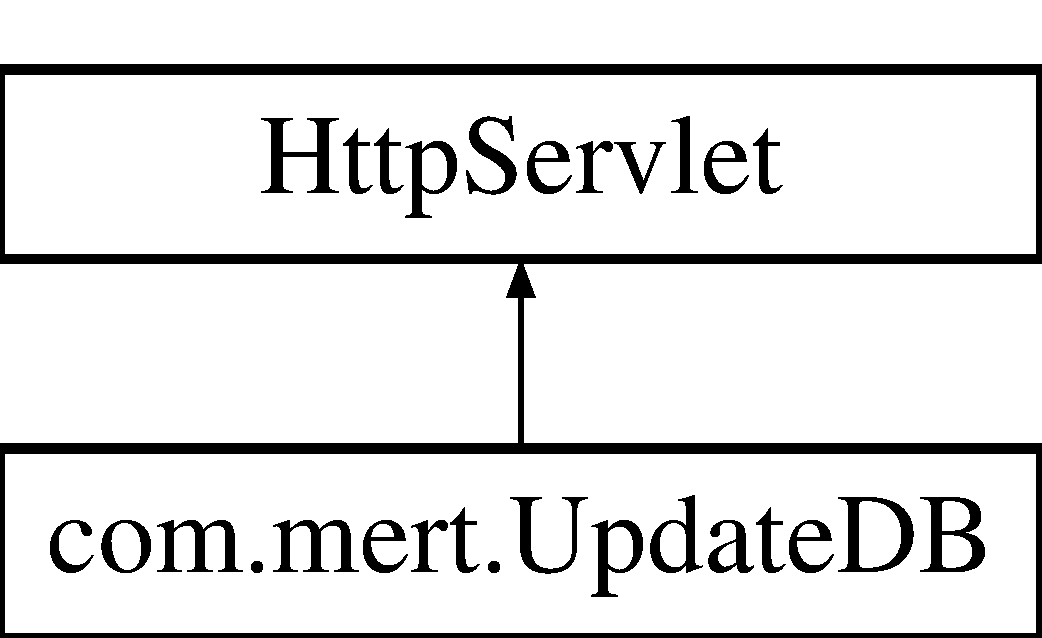
\includegraphics[height=2.000000cm]{classcom_1_1mert_1_1_update_d_b}
\end{center}
\end{figure}
\subsection*{Public Member Functions}
\begin{DoxyCompactItemize}
\item 
int \hyperlink{classcom_1_1mert_1_1_update_d_b_abdd8ebc75cea7ddd5ec0e5209fe33aab}{parse\+Count} (String s)
\item 
String \hyperlink{classcom_1_1mert_1_1_update_d_b_abb3f580bac381c22f673cb8ea31cd98c}{parse\+Link} (String s)
\item 
void \hyperlink{classcom_1_1mert_1_1_update_d_b_ac0ad352f8b973b5d27acd72ad42f9028}{truncate\+DB} ()
\end{DoxyCompactItemize}
\subsection*{Static Public Member Functions}
\begin{DoxyCompactItemize}
\item 
static String \hyperlink{classcom_1_1mert_1_1_update_d_b_a318392aaae286a267a142550bdd78ca0}{parse\+Genre} (String s)
\end{DoxyCompactItemize}
\subsection*{Protected Member Functions}
\begin{DoxyCompactItemize}
\item 
void \hyperlink{classcom_1_1mert_1_1_update_d_b_abd05581f8da7d00b5d3cb2326f592dab}{do\+Get} (Http\+Servlet\+Request request, Http\+Servlet\+Response response)  throws Servlet\+Exception, I\+O\+Exception 
\item 
void \hyperlink{classcom_1_1mert_1_1_update_d_b_a8c87bdcc44be032b163f3d996d230585}{do\+Post} (Http\+Servlet\+Request request, Http\+Servlet\+Response response)  throws Servlet\+Exception, I\+O\+Exception 
\end{DoxyCompactItemize}


\subsection{Detailed Description}
Queries the wikidata.\+org to get up-\/to-\/date information and stores it in local DB \begin{DoxyAuthor}{Author}
Mert 
\end{DoxyAuthor}


\subsection{Member Function Documentation}
\index{com\+::mert\+::\+Update\+DB@{com\+::mert\+::\+Update\+DB}!do\+Get@{do\+Get}}
\index{do\+Get@{do\+Get}!com\+::mert\+::\+Update\+DB@{com\+::mert\+::\+Update\+DB}}
\subsubsection[{\texorpdfstring{do\+Get(\+Http\+Servlet\+Request request, Http\+Servlet\+Response response)}{doGet(HttpServletRequest request, HttpServletResponse response)}}]{\setlength{\rightskip}{0pt plus 5cm}void com.\+mert.\+Update\+D\+B.\+do\+Get (
\begin{DoxyParamCaption}
\item[{Http\+Servlet\+Request}]{request, }
\item[{Http\+Servlet\+Response}]{response}
\end{DoxyParamCaption}
) throws Servlet\+Exception, I\+O\+Exception\hspace{0.3cm}{\ttfamily [protected]}}\hypertarget{classcom_1_1mert_1_1_update_d_b_abd05581f8da7d00b5d3cb2326f592dab}{}\label{classcom_1_1mert_1_1_update_d_b_abd05581f8da7d00b5d3cb2326f592dab}
\begin{DoxySeeAlso}{See also}
Http\+Servlet\+::do\+Get(Http\+Servlet\+Request request, Http\+Servlet\+Response response) 
\end{DoxySeeAlso}
\index{com\+::mert\+::\+Update\+DB@{com\+::mert\+::\+Update\+DB}!do\+Post@{do\+Post}}
\index{do\+Post@{do\+Post}!com\+::mert\+::\+Update\+DB@{com\+::mert\+::\+Update\+DB}}
\subsubsection[{\texorpdfstring{do\+Post(\+Http\+Servlet\+Request request, Http\+Servlet\+Response response)}{doPost(HttpServletRequest request, HttpServletResponse response)}}]{\setlength{\rightskip}{0pt plus 5cm}void com.\+mert.\+Update\+D\+B.\+do\+Post (
\begin{DoxyParamCaption}
\item[{Http\+Servlet\+Request}]{request, }
\item[{Http\+Servlet\+Response}]{response}
\end{DoxyParamCaption}
) throws Servlet\+Exception, I\+O\+Exception\hspace{0.3cm}{\ttfamily [protected]}}\hypertarget{classcom_1_1mert_1_1_update_d_b_a8c87bdcc44be032b163f3d996d230585}{}\label{classcom_1_1mert_1_1_update_d_b_a8c87bdcc44be032b163f3d996d230585}
\begin{DoxySeeAlso}{See also}
Http\+Servlet\+::do\+Post(Http\+Servlet\+Request request, Http\+Servlet\+Response response) 
\end{DoxySeeAlso}
\index{com\+::mert\+::\+Update\+DB@{com\+::mert\+::\+Update\+DB}!parse\+Count@{parse\+Count}}
\index{parse\+Count@{parse\+Count}!com\+::mert\+::\+Update\+DB@{com\+::mert\+::\+Update\+DB}}
\subsubsection[{\texorpdfstring{parse\+Count(\+String s)}{parseCount(String s)}}]{\setlength{\rightskip}{0pt plus 5cm}int com.\+mert.\+Update\+D\+B.\+parse\+Count (
\begin{DoxyParamCaption}
\item[{String}]{s}
\end{DoxyParamCaption}
)}\hypertarget{classcom_1_1mert_1_1_update_d_b_abdd8ebc75cea7ddd5ec0e5209fe33aab}{}\label{classcom_1_1mert_1_1_update_d_b_abdd8ebc75cea7ddd5ec0e5209fe33aab}
Parses the retrieved \char`\"{}count\char`\"{} string and turns it into the integer before character \char`\"{}$^\wedge$\char`\"{} 
\begin{DoxyParams}{Parameters}
{\em s} & String to be parsed \\
\hline
\end{DoxyParams}
\begin{DoxyReturn}{Returns}
count as integer 
\end{DoxyReturn}
\index{com\+::mert\+::\+Update\+DB@{com\+::mert\+::\+Update\+DB}!parse\+Genre@{parse\+Genre}}
\index{parse\+Genre@{parse\+Genre}!com\+::mert\+::\+Update\+DB@{com\+::mert\+::\+Update\+DB}}
\subsubsection[{\texorpdfstring{parse\+Genre(\+String s)}{parseGenre(String s)}}]{\setlength{\rightskip}{0pt plus 5cm}static String com.\+mert.\+Update\+D\+B.\+parse\+Genre (
\begin{DoxyParamCaption}
\item[{String}]{s}
\end{DoxyParamCaption}
)\hspace{0.3cm}{\ttfamily [static]}}\hypertarget{classcom_1_1mert_1_1_update_d_b_a318392aaae286a267a142550bdd78ca0}{}\label{classcom_1_1mert_1_1_update_d_b_a318392aaae286a267a142550bdd78ca0}
Parses the retrieved \char`\"{}genre\char`\"{} string and turns it into the integer before character \char`\"{}@\char`\"{} 
\begin{DoxyParams}{Parameters}
{\em s} & String to be parsed \\
\hline
\end{DoxyParams}
\begin{DoxyReturn}{Returns}
genre as string 
\end{DoxyReturn}
\index{com\+::mert\+::\+Update\+DB@{com\+::mert\+::\+Update\+DB}!parse\+Link@{parse\+Link}}
\index{parse\+Link@{parse\+Link}!com\+::mert\+::\+Update\+DB@{com\+::mert\+::\+Update\+DB}}
\subsubsection[{\texorpdfstring{parse\+Link(\+String s)}{parseLink(String s)}}]{\setlength{\rightskip}{0pt plus 5cm}String com.\+mert.\+Update\+D\+B.\+parse\+Link (
\begin{DoxyParamCaption}
\item[{String}]{s}
\end{DoxyParamCaption}
)}\hypertarget{classcom_1_1mert_1_1_update_d_b_abb3f580bac381c22f673cb8ea31cd98c}{}\label{classcom_1_1mert_1_1_update_d_b_abb3f580bac381c22f673cb8ea31cd98c}
Parses the retrieved \char`\"{}link\char`\"{} string and takes the last ID part 
\begin{DoxyParams}{Parameters}
{\em s} & String to be parsed \\
\hline
\end{DoxyParams}
\begin{DoxyReturn}{Returns}
ID as string i.\+e Q342 
\end{DoxyReturn}
\index{com\+::mert\+::\+Update\+DB@{com\+::mert\+::\+Update\+DB}!truncate\+DB@{truncate\+DB}}
\index{truncate\+DB@{truncate\+DB}!com\+::mert\+::\+Update\+DB@{com\+::mert\+::\+Update\+DB}}
\subsubsection[{\texorpdfstring{truncate\+D\+B()}{truncateDB()}}]{\setlength{\rightskip}{0pt plus 5cm}void com.\+mert.\+Update\+D\+B.\+truncate\+DB (
\begin{DoxyParamCaption}
{}
\end{DoxyParamCaption}
)}\hypertarget{classcom_1_1mert_1_1_update_d_b_ac0ad352f8b973b5d27acd72ad42f9028}{}\label{classcom_1_1mert_1_1_update_d_b_ac0ad352f8b973b5d27acd72ad42f9028}
Deletes all entries from the local DB 

The documentation for this class was generated from the following file\+:\begin{DoxyCompactItemize}
\item 
src/com/mert/Update\+D\+B.\+java\end{DoxyCompactItemize}

%--- End generated contents ---

% Index
\backmatter
\newpage
\phantomsection
\clearemptydoublepage
\addcontentsline{toc}{chapter}{Index}
\printindex

\end{document}
